% !TeX root = cm1015-cm-notes.tex

\documentclass{article}
\usepackage[utf8]{inputenc}
\usepackage[english]{babel}
\usepackage{xcolor}

\usepackage{minted}
\setminted{fontfamily=tt}
% Disable italics for comments and configure color of code block text
\usepackage{etoolbox}
\BeforeBeginEnvironment{minted}{\def\FancyVerbFormatLine{\def\baselinestretch{1}\small\color{white}}}
\AtBeginEnvironment{minted}{\let\itshape\relax}

\usepackage{graphicx}
\usepackage{tikz}

\usepackage[scaled]{helvet}
\renewcommand*\familydefault{\sfdefault}

\usepackage[hmargin=2.54cm, vmargin=2.54cm]{geometry}

% Define custom color
\definecolor{darkgray}{RGB}{13, 17, 23}
\definecolor{lightgrey}{RGB}{216, 222, 233}

\pagecolor{darkgray}
\color{lightgrey}

\begin{document}

\begin{titlepage}
    \centering
    \vspace*{2cm}
    
    {\LARGE\bfseries CM1015 - Computational Mathematics}\\[0.8cm]
    {\large\bfseries BSc Computer Science}\\[0.5cm] 
    {\large\textnormal{Nathan Donovan}}\\[1.5cm] 

    
\includegraphics[scale=0.1]{../images/university-of-london-logo.png}\\[1.5cm] 
    {\Large\bfseries University of London}\\[1cm]
    {\large April 2024}

    \vfill
    
\end{titlepage}

\newpage
\section*{Number Bases}
\subsection*{Decimal}

\noindent Number bases relate to the amount of digits used to represent a number. 
The decimal system is base 10, meaning it uses 10 digits (0-9) to represent numbers. 
The value of a number is calculated by multiplying each digit by the base raised to the power of its position. 
For example, the number 123 in decimal is calculated as follows:

\vspace{0.5cm}

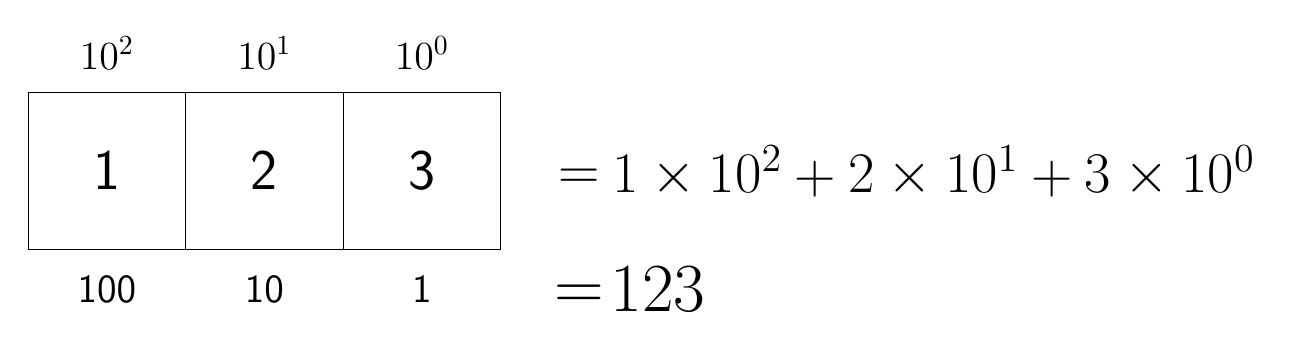
\begin{tikzpicture}
    \foreach \x/\y/\base/\dec in {0/1/2/100, 2/2/1/10, 4/3/0/1} {
        % Base value above the square
        \node at (\x,2.5) {\Large$10^{\base}$};
        % Draw the larger square
        \draw (\x-1,0) rectangle ++(2,2);
        % Number inside the square
        \node at (\x,1) {\huge \y};
        % Decimal value below the square
        \node at (\x,-0.5) {\Large\dec};
    }
    \node at (6,0.9) {\huge $=$};
    \node at (7.5,1) {\huge $1 \times 10^2$};
    \node at (9,0.9) {\huge $+$};
    \node at (10.5,1) {\huge $2 \times 10^1$};
    \node at (12,0.9) {\huge $+$};
    \node at (13.5,1) {\huge $3 \times 10^0$};

    \node at (6,-0.6) {\Huge $=$};
    \node at (7,-0.5) {\Huge $123$};
\end{tikzpicture}

\vspace*{0.5cm}

\subsection*{Binary}

\noindent The binary system is base 2, meaning it uses 2 digits (0-1) to represent numbers. Binary numbers are calculated in the same way as decimal numbers, but using powers of 2 instead of 10. For example, the binary number 101 in decimal is calculated as follows:

\vspace*{0.5cm}

\begin{tikzpicture}
    \foreach \x/\y/\base/\dec in {0/1/2/4, 2/0/1/2, 4/1/0/1} {
        % Base value above the square
        \node at (\x,2.5) {\Large$2^{\base}$};
        % Draw the larger square
        \draw (\x-1,0) rectangle ++(2,2);
        % Number inside the square
        \node at (\x,1) {\huge \y};
        % Decimal value below the square
        \node at (\x,-0.5) {\Large\dec};
    }
    \node at (6,0.9) {\huge $=$};
    \node at (7.5,1) {\huge $1 \times 2^2$};
    \node at (9,0.9) {\huge $+$};
    \node at (10.5,1) {\huge $0 \times 2^1$};
    \node at (12,0.9) {\huge $+$};
    \node at (13.5,1) {\huge $1 \times 2^0$};

    \node at (6,-0.6) {\Huge $=$};
    \node at (7,-0.5) {\Huge $5$};
\end{tikzpicture}

\vspace*{0.5cm}

\subsection*{Hexadecimal}

\noindent The hexadecimal system is base 16, meaning it uses 16 digits (0-9, A-F) to represent numbers. Hexadecimal numbers are calculated in the same way as decimal numbers, but using powers of 16 instead of 10. For example, the hexadecimal number 1A3 in decimal is calculated as follows:

\vspace*{0.5cm}

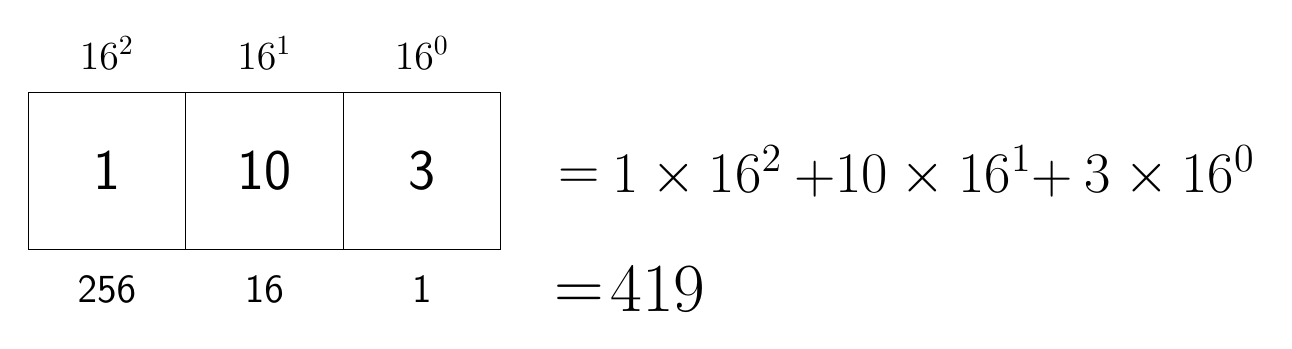
\begin{tikzpicture}
    \foreach \x/\y/\base/\dec in {0/1/2/256, 2/10/1/16, 4/3/0/1} {
        % Base value above the square
        \node at (\x,2.5) {\Large$16^{\base}$};
        % Draw the larger square
        \draw (\x-1,0) rectangle ++(2,2);
        % Number inside the square
        \node at (\x,1) {\huge \y};
        % Decimal value below the square
        \node at (\x,-0.5) {\Large\dec};
    }
    \node at (6,0.9) {\huge $=$};
    \node at (7.5,1) {\huge $1 \times 16^2$};
    \node at (9,0.9) {\huge $+$};
    \node at (10.5,1) {\huge $10 \times 16^1$};
    \node at (12,0.9) {\huge $+$};
    \node at (13.5,1) {\huge $3 \times 16^0$};

    \node at (6,-0.6) {\Huge $=$};
    \node at (7,-0.5) {\Huge $419$};
\end{tikzpicture}

\newpage

\subsection*{Generic Base Conversion to Decimal}

\noindent To convert any base to decimal, the following method can be used:

\begin{enumerate}
    \item Write the number in the base you are converting from.
    \item Multiply each digit by the base raised to the power of its position.
    \item Add the results together to get the decimal value.
\end{enumerate}

\vspace*{0.25cm}

\noindent Formula: $d_n \times b^n + d_{n-1} \times b^{n-1} + \ldots + d_1 \times b^1 + d_0 \times b^0$

\vspace*{0.25cm}

\noindent Where: $d_n$ is the digit at position $n$, $b$ is the base, and $n$ is the position of the digit.

\vspace*{0.25cm}

\noindent Example, shown with above symbols:

\vspace*{0.5cm}

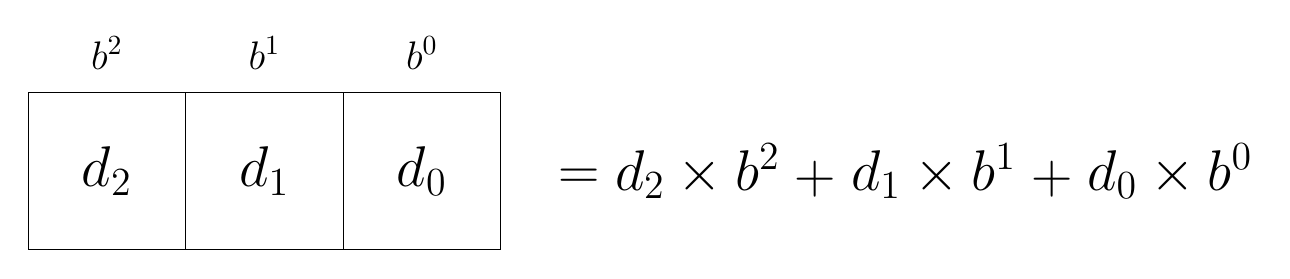
\begin{tikzpicture}
    \foreach \x/\y/\base/\dec in {0/1/2/4, 2/0/1/2, 4/1/0/1} {
        % Base value above the square
        \node at (\x,2.5) {\Large$b^{\base}$};
        % Draw the larger square
        \draw (\x-1,0) rectangle ++(2,2);
        % Number inside the square
        \node at (\x,1) {\huge $d_{\base}$};
    }
    \node at (6,0.9) {\huge $=$};
    \node at (7.5,1) {\huge $d_2 \times b^2$};
    \node at (9,0.9) {\huge $+$};
    \node at (10.5,1) {\huge $d_1 \times b^1$};
    \node at (12,0.9) {\huge $+$};
    \node at (13.5,1) {\huge $d_0 \times b^0$};

\end{tikzpicture}

\vspace*{0.5cm}

\noindent Example with base 5 number 234, here $b=5$, $d_2=2$, $d_1=3$, $d_0=4$:

\vspace*{0.5cm}

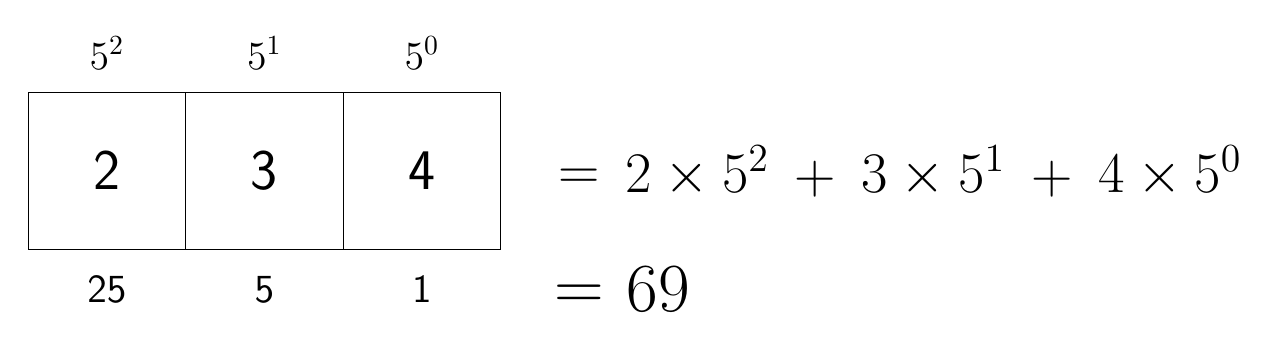
\begin{tikzpicture}
    \foreach \x/\y/\base/\dec in {0/2/2/25, 2/3/1/5, 4/4/0/1} {
        % Base value above the square
        \node at (\x,2.5) {\Large$5^{\base}$};
        % Draw the larger square
        \draw (\x-1,0) rectangle ++(2,2);
        % Number inside the square
        \node at (\x,1) {\huge \y};
        % Decimal value below the square
        \node at (\x,-0.5) {\Large\dec};
    }
    \node at (6,0.9) {\huge $=$};
    \node at (7.5,1) {\huge $2 \times 5^2$};
    \node at (9,0.9) {\huge $+$};
    \node at (10.5,1) {\huge $3 \times 5^1$};
    \node at (12,0.9) {\huge $+$};
    \node at (13.5,1) {\huge $4 \times 5^0$};

    \node at (6,-0.6) {\Huge $=$};
    \node at (7,-0.5) {\Huge $69$};
\end{tikzpicture}

\newpage

\subsection*{Non-integer Conversion to Decimal}

\noindent To convert a non-integer number to decimal, the following method can be used:

\begin{enumerate}
    \item Write the number in the base you are converting from.
    \item Multiply each digit by the base raised to the power of its position.
    \item Add the results together to get the integer part of the decimal value.
    \item Repeat the process for the fractional part of the number.
\end{enumerate}

\vspace*{0.25cm}

\noindent Formula: $d_n \times b^n + d_{n-1} \times b^{n-1} + \ldots + d_1 \times b^1 + d_0 \times b^0 + d_{-1} \times b^{-1} + d_{-2} \times b^{-2} + \ldots$

\vspace*{0.25cm}

\noindent Where: $d_n$ is the digit at position $n$, $b$ is the base, and $n$ is the position of the digit.

\vspace*{0.25cm}

\noindent Example, shown with above symbols:

\vspace*{0.5cm}

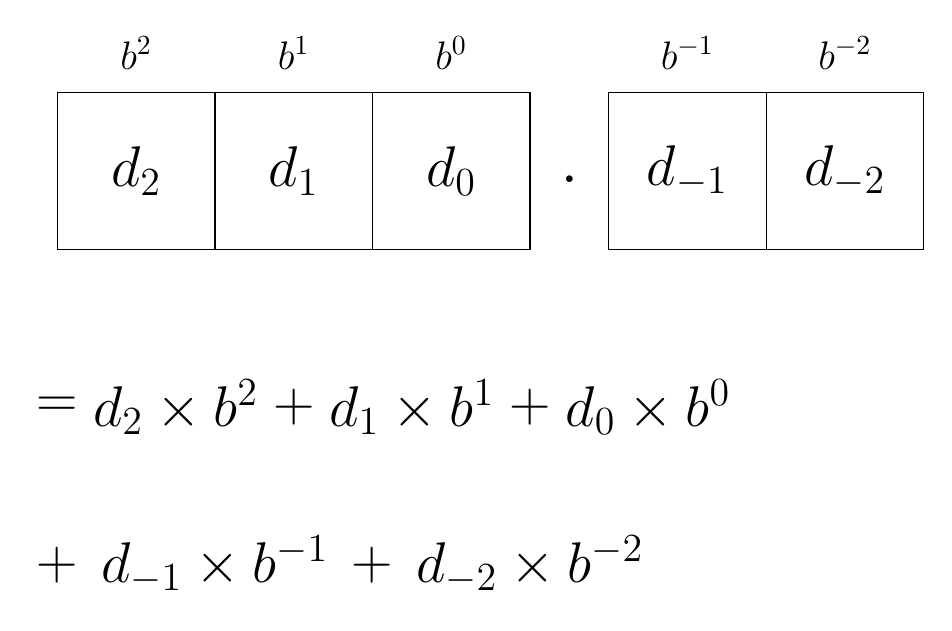
\begin{tikzpicture}
    \foreach \x/\y/\base/\dec in {0/1/2/4, 2/0/1/2, 4/1/0/1} {
        % Base value above the square
        \node at (\x,2.5) {\Large$b^{\base}$};
        % Draw the larger square
        \draw (\x-1,0) rectangle ++(2,2);
        % Number inside the square
        \node at (\x,1) {\huge $d_{\base}$};
    }

    \node at (5.5,0.9) {\Huge $.$};

    \foreach \x/\y/\base/\dec in {7/./-1/0.5, 9/1/-2/0.25} {
        % Base value above the square
        \node at (\x,2.5) {\Large$b^{\base}$};
        % Draw the larger square
        \draw (\x-1,0) rectangle ++(2,2);
        % Number inside the square
        \node at (\x,1) {\huge $d_{\base}$};
    }

    \node at (-1,-2) {\huge $=$};
    \node at (0.5,-2) {\huge $d_2 \times b^2$};
    \node at (2,-2) {\huge $+$};
    \node at (3.5,-2) {\huge $d_1 \times b^1$};
    \node at (5,-2) {\huge $+$};
    \node at (6.5,-2) {\huge $d_0 \times b^0$};
    \node at (-1,-4) {\huge $+$};
    \node at (1,-4) {\huge $d_{-1} \times b^{-1}$};
    \node at (3,-4) {\huge $+$};
    \node at (5,-4) {\huge $d_{-2} \times b^{-2}$};

\end{tikzpicture}

\vspace*{0.5cm}

\noindent Example with base 5 number 234.25, here $b=5$, $d_2=2$, $d_1=3$, $d_0=4$, $d_{-1}=2$, $d_{-2}=5$:

\vspace*{0.5cm}

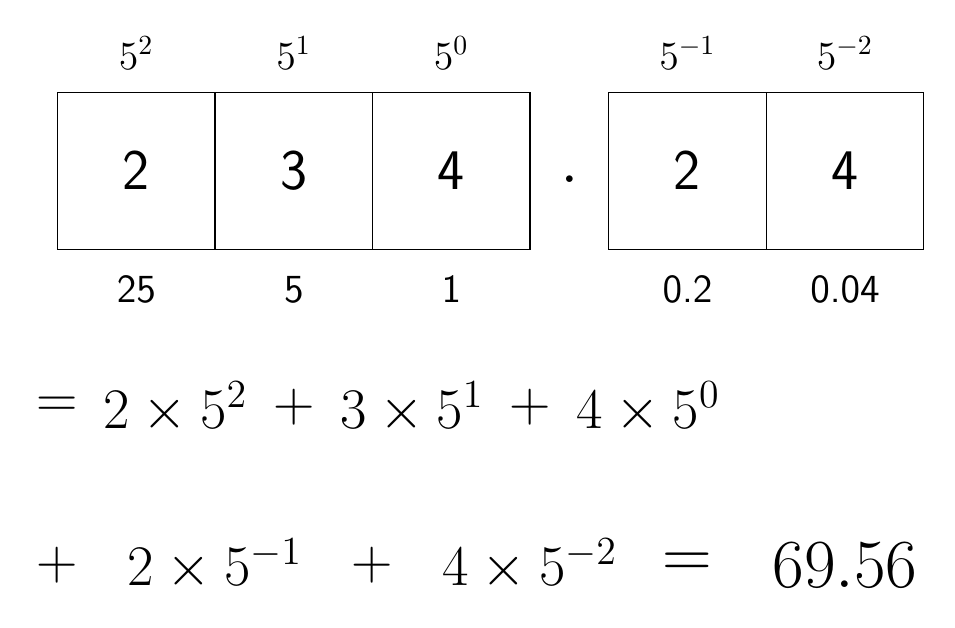
\begin{tikzpicture}
    \foreach \x/\y/\base/\dec in {0/2/2/25, 2/3/1/5, 4/4/0/1} {
        % Base value above the square
        \node at (\x,2.5) {\Large$5^{\base}$};
        % Draw the larger square
        \draw (\x-1,0) rectangle ++(2,2);
        % Number inside the square
        \node at (\x,1) {\huge \y};
        % Decimal value below the square
        \node at (\x,-0.5) {\Large\dec};
    }

    \node at (5.5,0.9) {\Huge $.$};

    \foreach \x/\y/\base/\dec in {7/2/-1/0.2, 9/4/-2/0.04} {
        % Base value above the square
        \node at (\x,2.5) {\Large$5^{\base}$};
        % Draw the larger square
        \draw (\x-1,0) rectangle ++(2,2);
        % Number inside the square
        \node at (\x,1) {\huge \y};
        % Decimal value below the square
        \node at (\x,-0.5) {\Large\dec};
    }

    \node at (-1,-2) {\huge $=$};
    \node at (0.5,-2) {\huge $2 \times 5^2$};
    \node at (2,-2) {\huge $+$};
    \node at (3.5,-2) {\huge $3 \times 5^1$};
    \node at (5,-2) {\huge $+$};
    \node at (6.5,-2) {\huge $4 \times 5^0$};
    \node at (-1,-4) {\huge $+$};
    \node at (1,-4) {\huge $2 \times 5^{-1}$};
    \node at (3,-4) {\huge $+$};
    \node at (5,-4) {\huge $4 \times 5^{-2}$};

    \node at (7,-4) {\Huge $=$};
    \node at (9,-4) {\Huge $69.56$};
\end{tikzpicture}



\newpage

\subsection*{Self-assessment Questions from Foundation Maths Book}
\subsubsection*{Worked Example 14.2} Convert $83_{10}$ to binary.

\vspace*{0.5cm}

\noindent \textbf{Solution:}

\vspace*{0.25cm}

\noindent The general method for converting a decimal number to binary is to repeatedly divide the number by 2 and record the remainder. 
The binary number is then read from the remainders in reverse order.

\vspace*{0.25cm}

\noindent The steps for converting 83 to binary are as follows:

\begin{enumerate}
    \item $83 \div 2 = 41$ remainder 1
    \item $41 \div 2 = 20$ remainder 1
    \item $20 \div 2 = 10$ remainder 0
    \item $10 \div 2 = 5$ remainder 0
    \item $5 \div 2 = 2$ remainder 1
    \item $2 \div 2 = 1$ remainder 0
    \item $1 \div 2 = 0$ remainder 1
    \item The binary number is read from the remainders in reverse order: $1010011$
\end{enumerate}

\vspace*{0.5cm}

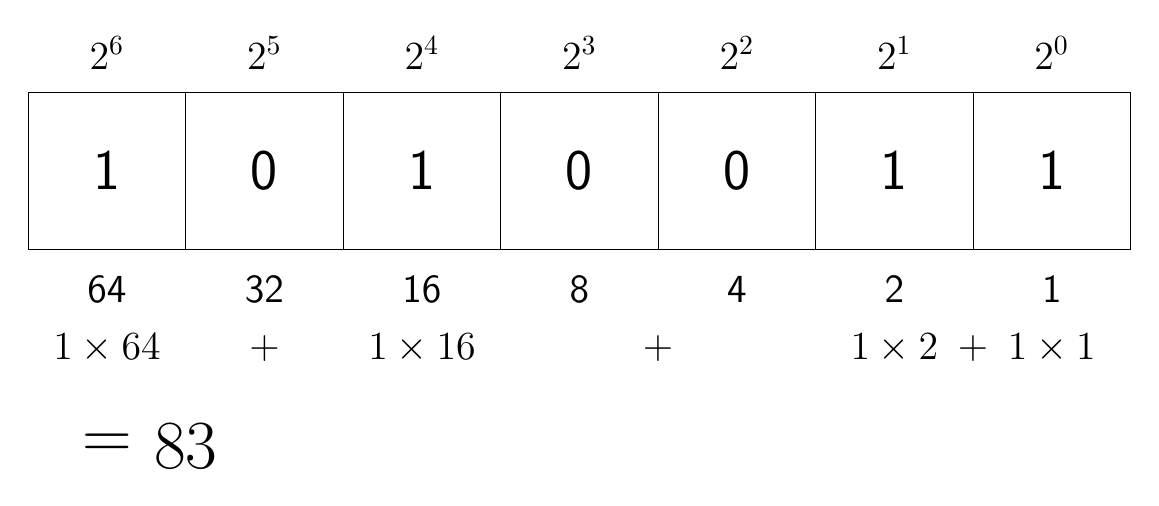
\begin{tikzpicture}
    \foreach \x/\y/\base/\dec in {0/1/6/64, 2/0/5/32, 4/1/4/16, 6/0/3/8, 8/0/2/4, 10/1/1/2, 12/1/0/1} {
        % Base value above the square
        \node at (\x,2.5) {\Large$2^{\base}$};
        % Draw the larger square
        \draw (\x-1,0) rectangle ++(2,2);
        % Number inside the square
        \node at (\x,1) {\huge \y};
        % Decimal value below the square
        \node at (\x,-0.5) {\Large\dec};
    }
    \node at (0,-1.25) {\Large $1 \times 64$};
    \node at (2,-1.25) {\Large $+$};
    \node at (4,-1.25) {\Large $1 \times 16$};
    \node at (7,-1.25) {\Large $+$};
    \node at (10,-1.25) {\Large $1 \times 2$};
    \node at (11,-1.25) {\Large $+$};
    \node at (12,-1.25) {\Large $1 \times 1$};

    \node at (0,-2.5) {\Huge $=$};
    \node at (1,-2.5) {\Huge $83$};

\end{tikzpicture}

\newpage

\subsubsection*{Exercise 14.2:} 
\vspace*{0.25cm}

\paragraph*{1.}
Convert the following decimal numbers to binary:

\vspace*{0.25cm}
(a): 19 (b): 36 (c): 100 (d): 796 (e): 5000

\vspace*{0.5cm}

\noindent \textbf{Solutions:}

\vspace*{0.25cm}

\noindent (a): $19_{10}$

\begin{enumerate}
    \item $19 \div 2 = 9$ remainder 1
    \item $9 \div 2 = 4$ remainder 1
    \item $4 \div 2 = 2$ remainder 0
    \item $2 \div 2 = 1$ remainder 0
    \item $1 \div 2 = 0$ remainder 1
    \item The binary number is read from the remainders in reverse order: $10011$
    \item $19_{10} = 10011_2$
    \item \textbf{Answer:} $19_{10} = 10011_2$
\end{enumerate}

\vspace*{0.5cm}

\noindent (b): $36_{10}$

\begin{enumerate}
    \item $36 \div 2 = 18$ remainder 0
    \item $18 \div 2 = 9$ remainder 0
    \item $9 \div 2 = 4$ remainder 1
    \item $4 \div 2 = 2$ remainder 0
    \item $2 \div 2 = 1$ remainder 0
    \item $1 \div 2 = 0$ remainder 1
    \item The binary number is read from the remainders in reverse order: $100100$
    \item $36_{10} = 100100_2$
    \item \textbf{Answer:} $36_{10} = 100100_2$
\end{enumerate}

\vspace*{0.5cm}

\noindent (c): $100_{10}$

\begin{enumerate}
    \item $100 \div 2 = 50$ remainder 0
    \item $50 \div 2 = 25$ remainder 0
    \item $25 \div 2 = 12$ remainder 1
    \item $12 \div 2 = 6$ remainder 0
    \item $6 \div 2 = 3$ remainder 0
    \item $3 \div 2 = 1$ remainder 1
    \item $1 \div 2 = 0$ remainder 1
    \item The binary number is read from the remainders in reverse order: $1100100$
    \item $100_{10} = 1100100_2$
    \item \textbf{Answer:} $100_{10} = 1100100_2$
\end{enumerate}

\vspace*{0.5cm}

\noindent (d): $796_{10}$

\begin{enumerate}
    \item $796 \div 2 = 398$ remainder 0
    \item $398 \div 2 = 199$ remainder 0
    \item $199 \div 2 = 99$ remainder 1
    \item $99 \div 2 = 49$ remainder 1
    \item $49 \div 2 = 24$ remainder 1
    \item $24 \div 2 = 12$ remainder 0
    \item $12 \div 2 = 6$ remainder 0
    \item $6 \div 2 = 3$ remainder 0
    \item $3 \div 2 = 1$ remainder 1
    \item $1 \div 2 = 0$ remainder 1
    \item The binary number is read from the remainders in reverse order: $1100011100$
    \item $796_{10} = 1100011100_2$
    \item \textbf{Answer:} $796_{10} = 1100011100_2$
\end{enumerate}

\vspace*{0.5cm}

\noindent (e): $5000_{10}$

\begin{enumerate}
    \item $5000 \div 2 = 2500$ remainder 0
    \item $2500 \div 2 = 1250$ remainder 0
    \item $1250 \div 2 = 625$ remainder 0
    \item $625 \div 2 = 312$ remainder 1
    \item $312 \div 2 = 156$ remainder 0
    \item $156 \div 2 = 78$ remainder 0
    \item $78 \div 2 = 39$ remainder 0
    \item $39 \div 2 = 19$ remainder 1
    \item $19 \div 2 = 9$ remainder 1
    \item $9 \div 2 = 4$ remainder 1
    \item $4 \div 2 = 2$ remainder 0
    \item $2 \div 2 = 1$ remainder 0
    \item $1 \div 2 = 0$ remainder 1
    \item The binary number is read from the remainders in reverse order: $1001110001000$
    \item $5000_{10} = 1001110001000_2$
    \item \textbf{Answer:} $5000_{10} = 1001110001000_2$
\end{enumerate}

\paragraph*{2.}
Convert the following binary numbers to decimal:

\vspace*{0.25cm}

(a): 111 (b): 10101 (c): 111001 (d): 1110001 (e): 11111111

\vspace*{0.5cm}

\noindent \textbf{Solutions:}

\vspace*{0.25cm}

\noindent (a): $111_2$

\begin{enumerate}
    \item $1 \times 2^2 + 1 \times 2^1 + 1 \times 2^0$
    \item $4 + 2 + 1 = 7$
    \item \textbf{Answer:} $111_2 = 7_{10}$
\end{enumerate}

\vspace*{0.5cm}

\noindent (b): $10101_2$

\begin{enumerate}
    \item $1 \times 2^4 + 0 \times 2^3 + 1 \times 2^2 + 0 \times 2^1 + 1 \times 2^0$
    \item $16 + 0 + 4 + 0 + 1 = 21$
    \item \textbf{Answer:} $10101_2 = 21_{10}$
\end{enumerate}

\vspace*{0.5cm}

\noindent (c): $111001_2$

\begin{enumerate}
    \item $1 \times 2^5 + 1 \times 2^4 + 1 \times 2^3 + 0 \times 2^2 + 0 \times 2^1 + 1 \times 2^0$
    \item $32 + 16 + 8 + 0 + 0 + 1 = 57$
    \item \textbf{Answer:} $111001_2 = 57_{10}$
\end{enumerate}

\vspace*{0.5cm}

\noindent (d): $1110001_2$

\begin{enumerate}
    \item $1 \times 2^6 + 1 \times 2^5 + 1 \times 2^4 + 0 \times 2^3 + 0 \times 2^2 + 0 \times 2^1 + 1 \times 2^0$
    \item $64 + 32 + 16 + 0 + 0 + 0 + 1 = 113$
    \item \textbf{Answer:} $1110001_2 = 113_{10}$
\end{enumerate}

\vspace*{0.5cm}

\noindent (e): $11111111_2$

\begin{enumerate}
    \item $1 \times 2^7 + 1 \times 2^6 + 1 \times 2^5 + 1 \times 2^4 + 1 \times 2^3 + 1 \times 2^2 + 1 \times 2^1 + 1 \times 2^0$
    \item $128 + 64 + 32 + 16 + 8 + 4 + 2 + 1 = 255$
    \item \textbf{Answer:} $11111111_2 = 255_{10}$
\end{enumerate}

\newpage

\paragraph*{3.}
What is the highest decimal number that can be written in binary form using a maximum of (a) two binary digits, 
(b) three binary digits, (c) four binary digits, (d) five binary digits? Can you spot a pattern? (e) Write a formula for 
the highest decimal number that can be written in binary form using $N$ binary digits.

\vspace*{0.5cm}

\noindent \textbf{Solutions:}

\vspace*{0.25cm}

\noindent (a): Two binary digits

\vspace*{0.25cm}

\noindent The highest decimal number that can be written in binary form using two binary digits is $11_2$, which is equal to $3_{10}$.

\vspace*{0.5cm}

\noindent (b): Three binary digits

\vspace*{0.25cm}

\noindent The highest decimal number that can be written in binary form using three binary digits is $111_2$, which is equal to $7_{10}$.

\vspace*{0.5cm}

\noindent (c): Four binary digits

\vspace*{0.25cm}

\noindent The highest decimal number that can be written in binary form using four binary digits is $1111_2$, which is equal to $15_{10}$.

\vspace*{0.5cm}

\noindent (d): Five binary digits

\vspace*{0.25cm}

\noindent The highest decimal number that can be written in binary form using five binary digits is $11111_2$, which is equal to $31_{10}$.

\vspace*{0.5cm}

\noindent (e): Formula for highest decimal number using $N$ binary digits

\vspace*{0.25cm}

\noindent The pattern observed is that the highest decimal number that can be written in binary form using $N$ binary digits is $2^N - 1$.

\vspace*{0.5cm}

\paragraph {4.}
Write the decimal number 0.5 in binary.

\vspace*{0.5cm}

\noindent \textbf{Solution:}

\vspace*{0.25cm}

\noindent The decimal number 0.5 can be written in binary as $0.1_2$.

\vspace*{0.5cm}

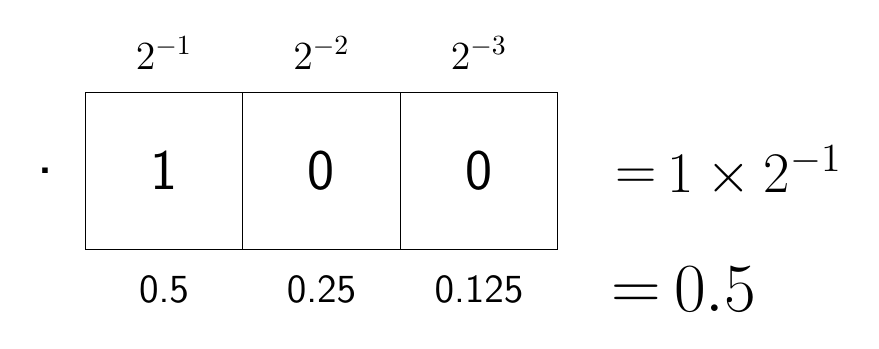
\begin{tikzpicture}
    \foreach \x/\y/\base/\dec in {0/1/1/0.5, 2/0/2/0.25, 4/0/3/0.125} {
        % Base value above the square
        \node at (\x,2.5) {\Large$2^{-\base}$};
        % Draw the larger square
        \draw (\x-1,0) rectangle ++(2,2);
        % Number inside the square
        \node at (\x,1) {\huge \y};
        % Decimal value below the square
        \node at (\x,-0.5) {\Large\dec};
    }
    \node at (6,0.9) {\huge $=$};
    \node at (7.5,1) {\huge $1 \times 2^{-1}$};
    \node at (6,-0.6) {\Huge $=$};
    \node at (7,-0.5) {\Huge $0.5$};
    \node at (-1.5,1) {\Huge .};
\end{tikzpicture}

\newpage

\subsubsection*{Exercise 14.3:}

\paragraph*{1.}
Convert the following decimal numbers to octal numbers:

\vspace*{0.25cm}

(a) 971 (b) 2841 (c) 5014 (d) 10000 (e) 17926

\vspace*{0.5cm}

\noindent \textbf{Solutions:}

\vspace*{0.25cm}

\noindent (a): $971_{10}$

\begin{enumerate}
    \item $971 \div 8 = 121$ remainder 3
    \item $121 \div 8 = 15$ remainder 1
    \item $15 \div 8 = 1$ remainder 7
    \item $1 \div 8 = 0$ remainder 1
    \item The octal number is read from the remainders in reverse order: $1733$
    \item $971_{10} = 1733_8$
    \item \textbf{Answer:} $971_{10} = 1733_8$
\end{enumerate}

\vspace*{0.5cm}

\noindent (b): $2841_{10}$

\begin{enumerate}
    \item $2841 \div 8 = 355$ remainder 1
    \item $355 \div 8 = 44$ remainder 3
    \item $44 \div 8 = 5$ remainder 4
    \item $5 \div 8 = 0$ remainder 5
    \item The octal number is read from the remainders in reverse order: $5431$
    \item $2841_{10} = 5431_8$
    \item \textbf{Answer:} $2841_{10} = 5431_8$
\end{enumerate}

\vspace*{0.5cm}

\noindent (c): $5014_{10}$

\begin{enumerate}
    \item $5014 \div 8 = 626$ remainder 6
    \item $626 \div 8 = 78$ remainder 2
    \item $78 \div 8 = 9$ remainder 6
    \item $9 \div 8 = 1$ remainder 1
    \item $1 \div 8 = 0$ remainder 1
    \item The octal number is read from the remainders in reverse order: $16126$
    \item $5014_{10} = 16126_8$
    \item \textbf{Answer:} $5014_{10} = 16126_8$
\end{enumerate}

\newpage

\noindent (d): $10000_{10}$

\begin{enumerate}
    \item $10000 \div 8 = 1250$ remainder 0
    \item $1250 \div 8 = 156$ remainder 2
    \item $156 \div 8 = 19$ remainder 4
    \item $19 \div 8 = 2$ remainder 3
    \item $2 \div 8 = 0$ remainder 2
    \item The octal number is read from the remainders in reverse order: $23420$
    \item $10000_{10} = 23420_8$
    \item \textbf{Answer:} $10000_{10} = 23420_8$
\end{enumerate}

\vspace*{0.5cm}

\noindent (e): $17926_{10}$

\begin{enumerate}
    \item $17926 \div 8 = 2240$ remainder 6
    \item $2240 \div 8 = 280$ remainder 0
    \item $280 \div 8 = 35$ remainder 0
    \item $35 \div 8 = 4$ remainder 3
    \item $4 \div 8 = 0$ remainder 4
    \item The octal number is read from the remainders in reverse order: $43006$
    \item $17926_{10} = 43006_8$
    \item \textbf{Answer:} $17926_{10} = 43006_8$
\end{enumerate}

\paragraph*{2.}

Convert the following octal numbers to decimal:

\vspace*{0.25cm}

(a) 73 (b) 1237 (c) 7635 (d) 6677 (e) 67765

\vspace*{0.5cm}

\noindent \textbf{Solutions:}

\vspace*{0.25cm}

\noindent (a): $73_8$

\begin{enumerate}
    \item $7 \times 8^1 + 3 \times 8^0$
    \item $56 + 3 = 59$
    \item \textbf{Answer:} $73_8 = 59_{10}$
\end{enumerate}

\vspace*{0.5cm}

\noindent (b): $1237_8$

\begin{enumerate}
    \item $1 \times 8^3 + 2 \times 8^2 + 3 \times 8^1 + 7 \times 8^0$
    \item $512 + 128 + 24 + 7 = 671$
    \item \textbf{Answer:} $1237_8 = 671_{10}$
\end{enumerate}

\newpage

\noindent (c): $7635_8$

\begin{enumerate}
    \item $7 \times 8^3 + 6 \times 8^2 + 3 \times 8^1 + 5 \times 8^0$
    \item $3584 + 384 + 24 + 5 = 3997$
    \item \textbf{Answer:} $7635_8 = 3997_{10}$
\end{enumerate}

\vspace*{0.5cm}

\noindent (d): $6677_8$

\begin{enumerate}
    \item $6 \times 8^3 + 6 \times 8^2 + 7 \times 8^1 + 7 \times 8^0$
    \item $3072 + 384 + 56 + 7 = 3519$
    \item \textbf{Answer:} $6677_8 = 3519_{10}$
\end{enumerate}

\vspace*{0.5cm}

\noindent (e): $67765_8$

\begin{enumerate}
    \item $6 \times 8^4 + 7 \times 8^3 + 7 \times 8^2 + 6 \times 8^1 + 5 \times 8^0$
    \item $24576 + 3584 + 448 + 48 + 5 = 28261$
    \item \textbf{Answer:} $67765_8 = 28261_{10}$
\end{enumerate}

\paragraph*{3.}

What is the highest decimal number that can be written in octal form using a maximum of 

(a) one digit, (b) two digits, (c) three digits, (d) four digits (e) five digits, (f) $N$ digits?

\vspace*{0.5cm}

\noindent \textbf{Solutions:}

\vspace*{0.25cm}

\noindent (a): One octal digit

\vspace*{0.25cm}

\noindent The highest decimal number that can be written in octal form using one octal digit is $7_8$, which is equal to $7_{10}$.

\vspace*{0.5cm}

\noindent (b): Two octal digits

\vspace*{0.25cm}

\noindent The highest decimal number that can be written in octal form using two octal digits is $77_8$, which is equal to $63_{10}$.

\vspace*{0.5cm}

\noindent (c): Three octal digits

\vspace*{0.25cm}

\noindent The highest decimal number that can be written in octal form using three octal digits is $777_8$, which is equal to $511_{10}$.

\vspace*{0.5cm}

\noindent (d): Four octal digits

\vspace*{0.25cm}

\noindent The highest decimal number that can be written in octal form using four octal digits is $7777_8$, which is equal to $4095_{10}$.

\vspace*{0.5cm}

\noindent (e): Five octal digits

\vspace*{0.25cm}

\noindent The highest decimal number that can be written in octal form using five octal digits is $77777_8$, which is equal to $32767_{10}$.

\vspace*{0.5cm}

\noindent (f): Formula for highest decimal number using $N$ octal digits

\vspace*{0.25cm}

\noindent The pattern observed is that the highest decimal number that can be written in octal form using $N$ octal digits is $8^N - 1$.

\newpage

\subsubsection*{Exercise 14.4:}

\paragraph*{1.}

Convert the following hexadecimal numbers to decimal:

(a) 91 (b) 6C (c) A1B (d) F9D4 (e) ABCD

\vspace*{0.5cm}

\noindent \textbf{Solutions:}

\vspace*{0.25cm}

\noindent (a): $91_{16}$

\begin{enumerate}
    \item $9 \times 16^1 + 1 \times 16^0$
    \item $144 + 1 = 145$
    \item \textbf{Answer:} $91_{16} = 145_{10}$
\end{enumerate}

\vspace*{0.5cm}

\noindent (b): $6C_{16}$

\begin{enumerate}
    \item $6 \times 16^1 + 12 \times 16^0$
    \item $96 + 12 = 108$
    \item \textbf{Answer:} $6C_{16} = 108_{10}$
\end{enumerate}

\vspace*{0.5cm}

\noindent (c): $A1B_{16}$

\begin{enumerate}
    \item $10 \times 16^2 + 1 \times 16^1 + 11 \times 16^0$
    \item $2560 + 16 + 11 = 2587$
    \item \textbf{Answer:} $A1B_{16} = 2587_{10}$
\end{enumerate}

\vspace*{0.5cm}

\noindent (d): $F9D4_{16}$

\begin{enumerate}
    \item $15 \times 16^3 + 9 \times 16^2 + 13 \times 16^1 + 4 \times 16^0$
    \item $61440 + 2304 + 208 + 4 = 63956$
    \item \textbf{Answer:} $F9D4_{16} = 63956_{10}$
\end{enumerate}

\vspace*{0.5cm}

\noindent (e): $ABCD_{16}$

\begin{enumerate}
    \item $10 \times 16^3 + 11 \times 16^2 + 12 \times 16^1 + 13 \times 16^0$
    \item $40960 + 2816 + 192 + 13 = 43981$
    \item \textbf{Answer:} $ABCD_{16} = 43981_{10}$
\end{enumerate}

\newpage

\paragraph*{2.}

Convert the following decimal numbers to hexadecimal:

(a) 160 (b) 396 (c) 5010 (d) 25000 (e) 1000000

\vspace*{0.5cm}

\noindent \textbf{Solutions:}

\vspace*{0.25cm}

\noindent (a): $160_{10}$

\begin{enumerate}
    \item $160 \div 16 = 10$ remainder 0
    \item $10 \div 16 = 0$ remainder 10
    \item The hexadecimal number is read from the remainders in reverse order: $A0$
    \item $160_{10} = A0_{16}$
    \item \textbf{Answer:} $160_{10} = A0_{16}$
\end{enumerate}

\vspace*{0.5cm}

\noindent (b): $396_{10}$

\begin{enumerate}
    \item $396 \div 16 = 24$ remainder 12
    \item $24 \div 16 = 1$ remainder 8
    \item $1 \div 16 = 0$ remainder 1
    \item The hexadecimal number is read from the remainders in reverse order: $18C$
    \item $396_{10} = 18C_{16}$
    \item \textbf{Answer:} $396_{10} = 18C_{16}$
\end{enumerate}

\vspace*{0.5cm}

\noindent (c): $5010_{10}$

\begin{enumerate}
    \item $5010 \div 16 = 313$ remainder 2
    \item $313 \div 16 = 19$ remainder 9
    \item $19 \div 16 = 1$ remainder 3
    \item $1 \div 16 = 0$ remainder 1
    \item The hexadecimal number is read from the remainders in reverse order: $1392$
    \item $5010_{10} = 1392_{16}$
    \item \textbf{Answer:} $5010_{10} = 1392_{16}$
\end{enumerate}

\newpage

\noindent (d): $25000_{10}$

\begin{enumerate}
    \item $25000 \div 16 = 1562$ remainder 8
    \item $1562 \div 16 = 97$ remainder 10
    \item $97 \div 16 = 6$ remainder 1
    \item $6 \div 16 = 0$ remainder 6
    \item The hexadecimal number is read from the remainders in reverse order: $61A8$
    \item $25000_{10} = 61A8_{16}$
    \item \textbf{Answer:} $25000_{10} = 61A8_{16}$
\end{enumerate}

\vspace*{0.5cm}

\noindent (e): $1000000_{10}$

\begin{enumerate}
    \item $1000000 \div 16 = 62500$ remainder 0
    \item $62500 \div 16 = 3906$ remainder 4
    \item $3906 \div 16 = 244$ remainder 2
    \item $244 \div 16 = 15$ remainder 4
    \item $15 \div 16 = 0$ remainder 15
    \item The hexadecimal number is read from the remainders in reverse order: $F4240$
    \item $1000000_{10} = F4240_{16}$
    \item \textbf{Answer:} $1000000_{10} = F4240_{16}$
\end{enumerate}

\paragraph*{3.}

Calculate the highest decimal number that can be represented by a hexadecimal with

(a) one digit, (b) two digits, (c) three digits, (d) four digits, (e) $N$ digits

\vspace*{0.5cm}

\noindent \textbf{Solutions:}

\vspace*{0.25cm}

\noindent (a): One hexadecimal digit

\vspace*{0.25cm}

\noindent The highest decimal number that can be represented by a hexadecimal with one hexadecimal digit is $F_{16}$, which is equal to $15_{10}$.

\vspace*{0.5cm}

\noindent (b): Two hexadecimal digits

\vspace*{0.25cm}

\noindent The highest decimal number that can be represented by a hexadecimal with two hexadecimal digits is $FF_{16}$, which is equal to $255_{10}$.

\vspace*{0.5cm}

\noindent (c): Three hexadecimal digits

\vspace*{0.25cm}

\noindent The highest decimal number that can be represented by a hexadecimal with three hexadecimal digits is $FFF_{16}$, which is equal to $4095_{10}$.

\newpage

\noindent (d): Four hexadecimal digits

\vspace*{0.25cm}

\noindent The highest decimal number that can be represented by a hexadecimal with four hexadecimal digits is $FFFF_{16}$, which is equal to $65535_{10}$.

\vspace*{0.5cm}

\noindent (e): $N$ hexadecimal digits

\vspace*{0.25cm}

\noindent The pattern observed is that the highest decimal number that can be represented by a hexadecimal with $N$ hexadecimal digits is $16^N - 1$.

\subsubsection {Challenge Exercise 14:}

\paragraph*{1.}

Convert the following decimal numbers to binary, octal and hexadecimal:

(a) 0.25 (b) 0.75

\vspace*{0.5cm}

\noindent \textbf{Solutions:}

\vspace*{0.25cm}

\noindent (a): $0.25_{10}$

\begin{enumerate}
    \item Binary: $0.01_2$
    \item Octal: $0.2_8$
    \item Hexadecimal: $0.4_{16}$
    \item \textbf{Answer:} $0.25_{10} = 0.01_2 = 0.2_8 = 0.4_{16}$
\end{enumerate}

\vspace*{0.5cm}

\noindent (b): $0.75_{10}$

\begin{enumerate}
    \item Binary: $0.11_2$
    \item Octal: $0.6_8$
    \item Hexadecimal: $0.C_{16}$
    \item \textbf{Answer:} $0.75_{10} = 0.11_2 = 0.6_8 = 0.C_{16}$
\end{enumerate}

\end{document}